
\chapter[Referencial Teórico]{Referencial Teórico}
Este capítulo apresenta os conceitos teóricos que abordam este trabalho, detalhando a estrutura cerebral responsável pela geração dos sinais de interesse na subseção 2.1, o sistema de captura dos sinais (a EEG) na subseção 2.2, o sistema que se refere às BCIs que realizam a tradução dos sinais em comandos para dispositivos na subseção 2.3, os detalhes técnicos a respeito dos sinais oferecidos pela base de dados \textit{BCI Competition} na subseção 2.4, a estrutura geral de um classificador LDA na subseção 2.5, os conceitos de um SoC na subseção 2.6 e por fim o estado da arte das implementações de algoritmos de classificação na subseção 2.7. 

\section{O Cérebro}
O Sistema Nervoso Central (SNC) é o responsável direto pelo comando do nosso comportamento geral\cite{David_Clarck}. Ele pode ser dividido em três principais áreas: tronco encefálico ou medula espinhal, o cérebro e o cerebelo (Figura \ref{BrainParts}) \cite{alvarezneurobiomecanismos}.

\begin{figure}[h]
	\centering
	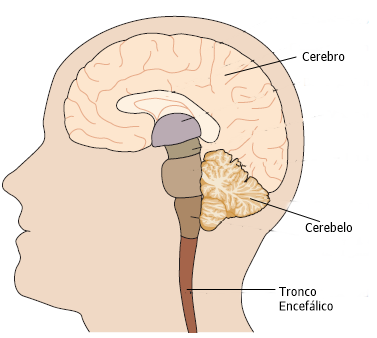
\includegraphics[keepaspectratio=true,scale=1.0]{figuras/estrutura_cerebral.PNG}
	\caption{Três principais áreas do cérebro \cite{alvarezneurobiomecanismos}}
	\label{BrainParts}
\end{figure}

O tronco encefálico, parte caldal do SNC recebe e processa todos os sinais dos sensores corporais, além de realizar o controle dos membros e do tronco humano \cite{KANDEL}.
O cérebro é o processador do SNC, nele são recebidos e processados os sinais da medula espinhal, além de fornecer todos os sinais de controle para a própria medula, que por sua vez distribui os sinais para os membros e tronco \cite{KANDEL}.
O cerebelo é localizado logo atrás do tronco encefálico que se conectam através de fibras chamadas de pedúnculos \cite{KANDEL}, é a segunda maior estrutura do SNC contendo mais da metade dos neurônios cerebrais, \cite{SIULYDissertacao} é responsável pelo mapeamento em volta do indivíduo, ou seja, sua percepção \cite{alvarezneurobiomecanismos}, além do controle da região motora e a memória de movimentos \cite{SIULYDissertacao,alvarezneurobiomecanismos}

\section{Eletroencefalografia}

\section{\textit{Brain Computer Interface}}

\section{\textit{BCI Competition}}
A \textit{BCI Competition} é uma competição que promove o desenvolvimento e melhoria da tecnologia voltada para as BCIs, onde são submetidas diferentes técnicas de análise de dados cerebrais \cite{BCICompetition}. Já foram realizadas quatro edições da competição, nos anos de 2001, 2002, 2004 e 2008 \cite{BCICompetition}. Em cada uma destas competições são fornecidos publicamente sinais cerebrais, adquiridos em laboratórios especializados \cite{BCICompetition}. Estes sinais são divididos em dois conjuntos de dados, os dados de treinamento e os dados de teste, que são utilizados para treinamento e teste dos algoritmos dos participantes \cite{BCICompetition}.

\subsection{\textit{BCI Competition III}}
O objetivo do \textit{BCI Competition III} é validar as metodologias de classificação e processamento de sinais cerebrais aplicados em BCIs desenvolvidas pelos participantes da competição \cite{siteBCI}. Esta edição foi realizada entre Maio e Junho de 2004, onde foram disponilizados 8 \textit{datasets} (I, II, II, IIIa, IIIb, IVa, IVb, IVc e V), desenvolvidos com a participação de 49 laboratórios especializados \cite{BCICompetition}.
Para cada um dos \textit{datasets} foram realizadas diferentes tarefas que estimulam atividades cerebrais durante a aquisição dos sinais, configurando assim um objetivo especifico para cada um dos \textit{datasets} \cite{siteBCI}.

\subsection{\textit{BCI Competition III - Dataset IVa}}
O \textit{dataset IVa} refere-se a um conjunto de dados adquiridos através da EEG, onde os sujeitos (indivíduos nos quais foram capturados os sinais) foram submetidos a estimular o cérebro por imagética motora, através de indicações visuais \cite{BCICompetition}. Os indivíduos foram submetidos a realizarem três tarefas, indicadas visualmente por 3.5s cada tarefa, sendo interrompidas em periodos aleatórios entre 1.75s e 2.25s, onde o sujeito era submetido a um periodo de relaxamento \cite{BCICompetition}. As três tarefas de imagéticas motoras foram: (L) mão esquerda, (R) mão direita e (F) pé direito \cite{BCICompetition}.

Foram adquiridos sinais de 5 sujeitos rotulados em \textit{aa, al, av, aw} e \textit{ay}, onde foram executadas no total 280 tarefas por cada sujeito, algumas previamente rotulada (dados de treinamento) em cada instante de tempo onde a tarefa foi executada, outras não rotuladas (dados de teste) \cite{siteBCI}. Estes sinais foram adquiridos, tratados e disponibilizados por \textit{Fraunhofer FIRST, Intelligent Data Analysis Group (Head: Klaus-Robert Müller), and Charité University Medicine Berlin, Campus Benjamin Franklin, Department of Neurology, Neurophysics Group} \cite{BCICompetition}. A tabela 1 apresenta a quantidade de tarefas previamente classificadas (nomeados \#tr) e a quantidade de tarefas não classificadas (nomeadas \#te) para cada sujeito.

\begin{table}[h!]
	\centering
	\caption{Número de tarefas rotuladas e não rotuladas por sujeito \cite{BCICompetition}.}
	\label{my-label}
	\begin{tabular}{lll}
		\textbf{Sujeitos} & \textbf{\#tr} & \textbf{\#te} \\
		\textit{aa} & 168 & 112 \\
		\textit{al} & 224 & 56 \\
		\textit{av} & 84 & 196 \\
		\textit{aw} & 56 & 224 \\
		\textit{ay} & 28 & 252
	\end{tabular}
\end{table}

Os dados foram adquiridos e armazenados utilizando amplificadores do tipo \textit{BrainAmp} e uma capa de eletrodos de 128 canais. Foram utilizados 118 canais de EEG posicionados de acordo com o sistema 10/20. Cada um destes canais foram filtrados em banda passante, utilizando um filtro \textit{butterworth} de quinta ordem entre as frequências de 0.05 e 200 Hz, posteriormente foram digitalizados com uma frequência de amostragem de 1 kHz com precisão de 16 bits, apresentando uma resolução de 0.1 $\mu$V, além disso tamém foram disponibilizados os mesmos dados com uma frequência de amostragem de 100 Hz \cite{siteBCI}.
 
\section{\textit{Linear Discriminant Analisys}}
Supondo a existência de um conjunto de dados L,com características multivariadas, e que cada dado
seja conhecido devido ser proveniente de uma das  classes K, tal que são predefinidas com características
semelhantes aos dados. As classes podem ser exemplificadas como sendo: espécies de plantas,
precença ou ausência de uma condição médica específica, diferentes tipos de tumores, tipos de veículos automotores
entre outros. Para separar as classes conhecidas uma das outras, é atribuido um rótulo a cada classe, então os dados são
representados como dados rotulados \cite{izenmanLDA}.


Devido a indispensabilidade de diminuir as dimensões dos dados de um determinado conjunto, o objetivo do LDA
é reduzir a dimensão do espaço de conjunto de dados, resolvendo o inconvêniente da sobreposição \cite{SinghLDA}.


\section{\textit{System-on-Chip}}

\textit{System-on-Chip} (SoC), implica que todo sistema que contém funcionalidades implementadas em hardware e software se encontra em um único chip de silício,combinando processamento, lógica de alta velocidade, interface, memória entre outros componentes ao invés de uma implementação maior em vários chips físicos diferentes agrupados em uma placa 
de cicuito impresso \cite{zynqBook}.

São vários os argumentos a favor da escolha de um SoC a uma placa de circuito impresso, pode-se citar que a solução é de menor custo, viabiliza transferência de dados mais rápidas e seguras entre vários elementos do sistema, possui maior velocidade geral do sistema, menor consumo de energia entre vários outros elementos que fortalecem a escolha de um SoC em sistemas discretos com componentes equivalentes \cite{zynqBook}.


\section{Estado da Arte}



